\newpage
\chapter{Theorie}
\label{sec:Theorie}
%\section{Theorie}
\section{Elementarstrahler}\label{sec:ElementareStrahler}
Die Funktionsart aller Antennen lässt sich auf die zwei Elementarstrahler Hertzscher Dipol und Fitzgeraldscher Dipol zurückführen. Ersterer stellt eine E-Feld Antenne, letzterer eine H-Feld Antenne dar. Die beiden Elementarstrahler dienen als theoretische Grundlage sämtlicher realer Antennen, können jedoch nicht praktisch angefertigt werden.

\section{Hertzscher Dipol}
Man kann sich den Hertzschen Dipol als eine sehr kurze Stabantenne vorstellen, bei welcher sich ein kurzer Stromfaden zwischen den beiden elektrischen Polen einstellt, dessen Stromrichtung von der Polarisierung der Dipole abhängt und somit mit der Kreisfrequenz $\omega $ die Richtung wechselt. Auf seiner gesamten Länge kann ein Strom mit der Amplitude $I$ und eine räumlich konstante Stromverteilung, die zeitlich sinusförmig schwingt, angenommen werden. Der Betrag des Dipolmoments \textit{p(t)} eines Hertzschen Dipols ist in (\ref{Dipolmoment}) beschrieben \cite{Emant}. 
\begin{equation}\label{Dipolmoment}
p(t)=pe^{j\omega t} = Q dl e^{j\omega t} = \frac{\hat{i} dl}{j\omega }e^{j\omega t}
\end{equation}
Aufgrund der Definition, dass ein Hertzscher Dipol als unendlich dünn ist, kann er als isotroper Punktstrahler betrachtet werden. In einem xyz-Koordinatensystem mit Ausrichtung des Dipols in z-Richtung bildet sich ein elektrisches Feld vom positiven zum negativen Ladungspunkt. Die Potentiale der Ladungspunkte oszillieren mit $\omega$. Die Ausrichtung der E-Feldlinien wechselt bei jeder Schwingung ihre Richtung. Im Nahfeld dominiert das E-Feld, weshalb der Hertzsche Dipol als elementaren elektrischen Dipol bezeichnet wird. Mit wachsendem Abstand von dem Strahler tritt zusätzlich ein magnetisches Feld auf. Dabei stehen das E-Feld und das H-Feld senkrecht zueinander und oszillieren in Phase. Sie können als ebene Wellenfront betrachtet werden. Die allgemeine Formel für die Feldverteilung im Kugelkoordinatensystem lautet \cite{elliott1981antenna}:
%\begin{center}
%\begin{minipage}{\linewidth}
%\centering
%\includegraphics{\conten\bilder\Herz_Dipol_EMANT_S37.pdf}%
%\captionof{figure}[kurze Bildunterschrift]{Bildunterschrift}%
%\end{minipage}
%\end{center}



%\begin{figure}[htbp]
%	\centering
%		\includegraphics[width=8cm]{content/Bilder/Z0_Grafik.png}
%	\caption{Wellenimpdedanz Z0}%
%	\label{Z0_Grafik}
%\end{figure}




\begin{equation}
E_r= \frac{I dl}{2\pi}   e^{-jkR} \left( \frac{n}{R^{2}}  + \frac{1}{j\omega \epsilon R^{3}}\right) cos(\theta)
\end{equation}

\begin{equation}
E_\theta= \frac{I dl}{4\pi}   e^{-jkR} \left( \frac{j\omega \mu}{R}  + \frac{n}{R^{2}}+ \frac{1}{j\omega \epsilon R^{3}}\right) sin(\theta)
\end{equation}

\begin{equation}
H_\varphi= \frac{I dl}{4\pi}   e^{-jkR} \left( \frac{jk}{R}  + \frac{n}{R^{2}}\right) sin(\theta)
\end{equation}

\begin{figure}[!ht]
	\centering
	\includegraphics[width=4cm]{content/bilder/HerzDipolEMANTS37.pdf}%
	\caption{Hertzscher Dipol mit dem Dipolmoment \textit{p(t)} \cite{Emant}}
	\label{HerzDipol}
\end{figure}


Mit wachsendem Abstand zur Strahlungsquelle können einige Terme vernachlässigt werden. Brüche mit dem  Abstand R in höherer Potenz als Nenner werden vereinfacht zu Null. Für das Fernfeld eines Hertzschen Dipols fergeben sich daher die folgenden Beschreibungen \cite{elliott1981antenna}:


\begin{equation}
E_r= 0
\end{equation}

\begin{equation}
E_\theta= \frac{I dl}{4\pi}   e^{-jkR} \left( \frac{j\omega \mu}{R}  \right) sin(\theta)
\end{equation}

\begin{equation}
H_\varphi= \frac{I dl}{4\pi}   e^{-jkR} \left( \frac{jk}{R} \right) sin(\theta)
\end{equation}
Im Fernfeld des Elementarstrahlers sind die Feldanteile von $E_r$ soweit abgeklungen, dass sie als Null angenommen werden. Es bleibt ein E-Feld Vektor und ein H-Feld Vektor übrig. Wie bereits erwähnt können die beiden E- und H-Vektoren als phasengleich und senkrecht zueinander angenommen werden. Sie werden sich soweit im Raum ausbreiten, bis ihre gesamte Energie absorbiert ist. Das bedeutet, die Amplituden der E- und H-Vektoren werden Null.\\


Für alle Antennen, welche eine lange und dünne Geometrie besitzen, wie zum Beispiel die Monopolantenne, die Dipol Antenne oder das Faltdipol, bildet der Hertzsche Dipol die theoretische Grundlage der Feldausbreitung. Die Ausdehnung des Elementarstrahlers ist auf eine Länge der strahlenden Struktur von etwa $100\mu m$ beschränkt. Da die Wellenlänge $\lambda$ der elektromagnetischen Strahlung bei einer Frequenz von ca. 3 THz 100$\mu m$ entspricht, reicht der Gültigkeitsbereich der in dieser Arbeit gezeigten Formeln und Beschreibungen bis zu einer Frequenz von 3 THz.
Die elektromagnetischen Felder eines Hertzschen Dipols werden oft in Kugelkoordinaten beschrieben. Jeder Punkt im Koordinatensystem kann mit einem Vektor $\vec{r}$ beschrieben werden, dessen Startpunkt im Ursprung des Koordinatensystems liegt. Der Vektor $\vec{r}$ kann in die xy Ebene projiziert werden. Der Winkel $\varphi$, gesprochen phi, bezeichnet die Abweichung des Vektors in Winkelgrad von der positiven x Achse. Er kann Werte von $\pm \pi$ erreichen und deckt somit $360^\circ$ ab. Der Winkel $\theta$, gesprochen theta, gibt die Neigung  des Vektors $\vec{r}$ zu der positiven z Achse an. Ein Vektor $\vec{r}$ ist in der Abbildung \ref{FerdVektor} gezeigt.




%%%%%%%%%%%%%%%%%%%%%%%%%%%%%%%%%%%
\begin{figure}[!ht]
\begin{center}
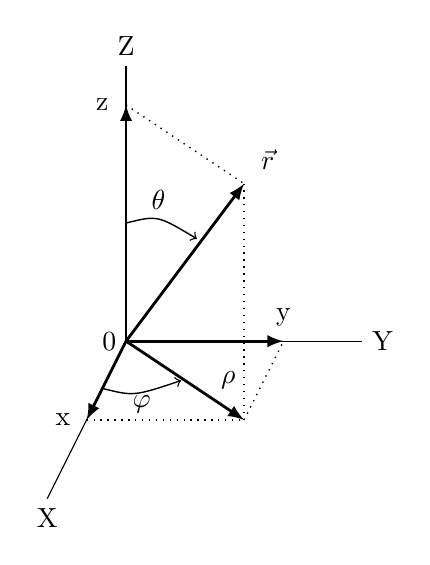
\begin{tikzpicture}
	\draw (4,4) -- (3,2) node[below] {X};%Fadenkreuz x
	\draw (4,4) node[left] {0} -- (7,4)node [right] {Y};%Fadenkreuz y
	\draw (4,4) -- (4,7.5) node[above] {Z};%Fadenkreuz z
	
	\draw[line width=1pt, ->, >=latex](4, 4)  -- (3.5, 3) node at (3.2, 3) {x};
	\draw[line width=1pt, ->, >=latex](4, 4)  -- (6, 4) node at (6, 4.3) {y};
	\draw[line width=1pt, ->, >=latex](4, 4)  -- (4, 7) node at (3.7, 7) {z};
	
	\draw[line width=0.5pt, style=dotted](3.5, 3) -- (5.5, 3);%Projektion y Rcihtung
	\draw[line width=0.5pt, style=dotted](5.5, 3) -- (6, 4);%Projektion x Rcihtung
	
	\draw[line width=1pt, ->, >=latex](4, 4)  -- (5.5, 3) node at (5.3, 3.5) {$\rho$};
	
	\draw[line width=1pt, ->, >=latex](4, 4)  -- (5.5, 6) node at (5.8, 6.3) {$\vec{r}$};
	
	\draw[line width=0.5pt, style=dotted](5.5, 3) -- (5.5, 6);%Projektion p zu \vec{r}
	\draw[line width=0.5pt, style=dotted](4, 7) -- (5.5, 6);%Projektion von z zur \vec{r}
	
	\coordinate (A) at (4, 5.5);
	\coordinate (B) at (4.9, 5.3);
	\coordinate (a) at (4.4, 5.6);
	\draw[line width=0.5pt, cap=round,->](A) .. controls (a) .. node[above] {$\theta$} (B);
	
	\coordinate (C) at (3.7, 3.4);
	\coordinate (D) at (4.7, 3.5);
	\coordinate (c) at (4.1, 3.3);
	\draw[line width=0.5pt, cap=round,->](C) .. controls (c) .. (D) node at (4.2, 3.2){$\varphi$};
\end{tikzpicture}
\end{center}
	\caption{Aufbau des Kugelkoordinatensystem}
	\label{FerdVektor}
\end{figure}

%%%%%%%%%%%%%%%%%%%%%%%%%%%%%%%%%%%%%%%%%%%%%%%%%%%%%%%%%%%%%%%%%%%

%%%%%%%%%%%%%%%%%%%%%%%%%%%%%%%%%%%%%%%%%%%%%%%%%%%%%%%%%%%%%%%%%%%
%\begin{figure}[h]
%\begin{center}
%\begin{tikzpicture}
%	\draw (4,4) -- (3,2)node at (3, 1.7) {X};%Fadenkreuz x
%	\draw (4,4) node[left] {0}-- (7,4)node at (7.3, 4) {Y};%Fadenkreuz y
%	\draw (4,4) -- (4,7.5)node at (3.7, 7.8) {Z};%Fadenkreuz z
%	
%	\draw[line width=1pt, ->, >=latex](4, 4)  -- (3.5, 3) node at (3.2, 3) {x};
%	\draw[line width=1pt, ->, >=latex](4, 4)  -- (6, 4) node at (6, 4.3) {y};
%	\draw[line width=1pt, ->, >=latex](4, 4)  -- (4, 7) node at (3.7, 7) {z};
%	
%	\draw[line width=0.5pt, style=dotted](3.5, 3) -- (5.5, 3);%Projektion y Rcihtung
%	\draw[line width=0.5pt, style=dotted](5.5, 3) -- (6, 4);%Projektion x Rcihtung
%	
%	\draw[line width=1pt, ->, >=latex](4, 4)  -- (5.5, 3) node at (5.3, 3.5) {$\rho$};
%	
%	\draw[line width=1pt, ->, >=latex](4, 4)  -- (5.5, 6) node at (5.5, 6.3) {$\vec{r}$};
%	
%	\draw[line width=0.5pt, style=dotted](5.5, 3) -- (5.5, 6);%Projektion p zu \vec{r}
%	\draw[line width=0.5pt, style=dotted](4, 7) -- (5.5, 6);%Projektion von z zur \vec{r}
%	
%	\coordinate (A) at (4, 5.5);
%	\coordinate (B) at (4.9, 5.3);
%	\coordinate (a) at (4.4, 5.6);
%	\draw[line width=0.5pt, cap=round,->](A) .. controls (a) .. (B) node at (4.4, 5.8){$\theta$};
%	
%	\coordinate (C) at (3.7, 3.4);
%	\coordinate (D) at (4.7, 3.5);
%	\coordinate (c) at (4.1, 3.3);
%	\draw[line width=0.5pt, cap=round,->](C) .. controls (c) .. (D) node at (4.2, 3.2){$\varphi$};
%	
%	%Einheitsvektoren
%	\draw[line width=1pt, ->, >=latex](5.5, 6)  -- (6.1, 6.8) node at (6.5, 7) {$\vec{E_{r}}\vec{e}$};
%	\draw[line width=1pt, ->, >=latex](5.5, 6)  -- (6.1, 5.6) node at (6.5, 5.4) {$\vec{E_{\theta}}\vec{e}$};
%	\draw[line width=1pt, ->, >=latex](5.5, 6)  -- (6.1, 6.3) node at (6.5, 6.1) {$\vec{H_{\varphi}}  \vec{e}$};
%	
%	%Antenne dipol
%	\draw[line width=3pt] (4,4.1) -- (4,5.2);
%	\draw[line width=3pt] (4,3.9) -- (4,2.8);
%\end{tikzpicture}
%\end{center}
%\caption{Dipolantanne mit Feldvektor und Einheitsvektoren}
%\label{DipolEFerdVektor}
%\end{figure}
%%%%%%%%%%%%%%%%%%%%%%%%%%%%%%%%%%%%%%%%%%%%%%%%%%%%%%%%%%%%%%%%%%%

\newpage
\section{Fitzgeraldscher Dipol }\label{sec:FitzgeraldescherDipol}
Dieser Dipol ist das Gegenstück zum Hertzschen Dipol und stellt somit den zweiten der beiden Elementarstrahler dar. Er besteht aus einer unendlich dünnen Leiterschleife, die auf der ganzen Länge dieselbe Stromverteilung besitzt. Es wird von einer Schleife gesprochen, da der Strom $I$ wie in einer Spule mit nur einer Windung geführt wird. Die Leiterschleife ist oft in der xy Ebene angeordnet. Da der Strom oszilliert, ist er als \textit{i(t)} gekennzeichnet. Der Strom \textit{i(t)} führt in einem Kreis im Abstand a um das Zentrum.
\begin{figure}[!h]
	\centering
	\includegraphics[width=5.2cm]{content/bilder/Fitzgerald_Dipol_EMANT_S37.pdf}%
	\caption{Fitzgeraldscher Dipol \cite{Emant}}
	\label{FitzDipol_elementar_Loop}
\end{figure}
\newpage 
Im Zentrum bildet sich ein magnetisches, zeitabhängiges Moment \textit{m(t)}. Stellt der Hertzsche Dipol eine E-Feld Antenne dar, so ist der Fitzgeraldsche Dipol eine H-Feld Antenne. In der unmittelbaren Nähe der Leitschleife bildet sich ein sehr starkes Magnetfeld aus. Das Nahfeld des Fitzgeraldschen Dipols wird mit den folgenden drei Formeln (\ref{Fitz_Nah_Hr}, \ref{Fitz_Nah_Etheta} und \ref{Fitz_Nah_Ephi}) beschrieben\cite{elliott1981antenna}:


\begin{equation}
H_r= \frac{I S}{2\pi}   e^{-jkR} \left( \frac{jk}{R^{2}}  + \frac{1}{R^{3}} \right) cos(\theta)
\label{Fitz_Nah_Hr}
\end{equation}

\begin{equation}
H_\theta= \frac{I S}{4\pi}   e^{-jkR} \left(- \frac{k^{2}}{R}  + \frac{jk}{R^{2}}+ \frac{1}{R^{3}} \right) sin(\theta)
\label{Fitz_Nah_Etheta}
\end{equation}

\begin{equation}
E_\phi= \frac{I S}{4\pi}   e^{-jkR} \left( \frac{k^{2}}{R}  - \frac{jk}{R^{2}} \right) sin(\theta)
\label{Fitz_Nah_Ephi}
\end{equation}
Das zeitabhängige magnetische Moment \textit{m(t)} ergibt sich durch die Multiplikation der durch die Windung aufgespannte Fläche $a^{2}\pi=S$ mit dem  Schleifenstrom $I$. Der Strom $I$ ist auf der ganzen Windung konstant. Dank der Annahme des konstanten Stroms kann wie in (\ref{eq:magnetischesMoment}) gezeigt, das magnetische Moment $m(t)$ berechnet werden \cite{Harrington-TimeHarmonic}: 
\begin{equation}\label{eq:magnetischesMoment}
Ia^{2}\pi=IS=m
\end{equation}
Wie beim Hertzschen Dipol können die Terme aus (\ref{Fitz_Nah_Hr}, \ref{Fitz_Nah_Etheta} und \ref{Fitz_Nah_Ephi}) mit R in der zweiten oder dritten Potenz als Nenner vernachlässigt werden für das Fernfeld. Die Amplituden des E- und H-Feldes sinken mit wachsendem Abstand $R$. Das Fernfeld kann daher wie folgt beschrieben werden:

\begin{equation}
H_r= 0
\end{equation}

\begin{equation}
H_\theta= \frac{I S}{4\pi}   e^{-jkR} \left(- \frac{k^{2}}{R}   \right) sin(\theta)
\end{equation}

\begin{equation}
E_\varphi= \frac{I S}{4\pi}   e^{-jkR} \left( \frac{k^{2}}{R}   \right) sin(\theta)
\end{equation}
Im Fernfeld fällt mit zunehmendem Abstand $R$ der Anteil  $H_r$ des magnetischen Feldes weg. Bis zur vollständigen Absorption der elektromagnetischen Wellen bei unendlich grossem Abstand $R$ bleiben die orthogonalen Feldvektoren $ E_\varphi $ und $ H_\theta $ erhalten.\\
Die Abbildung \ref{LoopFerdVektor} zeigt eine Fitzgeraldscher Dipol als Leiterschleife in der xy Ebene. Sein Zentrum bildet der Ursprung des Koordinatensystems und ist mit Null gekennzeichnet. Ebenfalls ist ein $\vec{r}$ mit entsprechenden Projektionslinien zur z-Achse und auf die xy-Ebene dargestellt. An der Spitze des $\vec{r}$ sind die Feldvektoren $H_{r}, H_{\theta}$ und $H_{\varphi}$ mit den entsprechenden Einheitsvektoren $\vec{e}$ gezeichnet.
%%%%%%%%%%%%%%%%%%%%%%%%%%%%%%%%%%%%%%%%%%%%%%%%%%%%%%%%%%%%%%%%%%%
\newpage

\begin{figure}[t]
\begin{center}
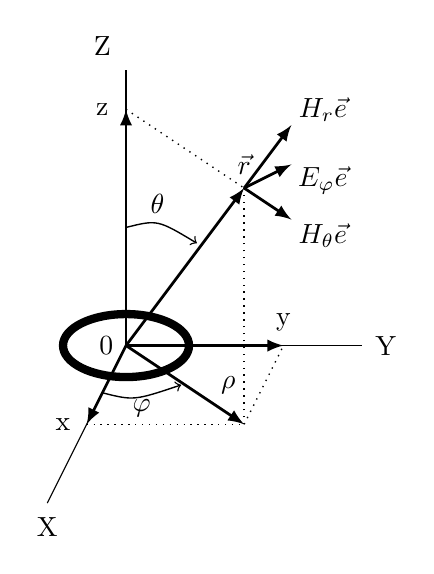
\begin{tikzpicture}
	\draw (4,4) -- (3,2)node at (3, 1.7) {X};%Fadenkreuz x
	\draw (4,4) node at(3.75,4) {0} -- (7,4)node at (7.3, 4) {Y};%Fadenkreuz y
	\draw (4,4) -- (4,7.5)node at (3.7, 7.8) {Z};%Fadenkreuz z
	
	\draw[line width=1pt, ->, >=latex](4, 4)  -- (3.5, 3) node at (3.2, 3) {x};
	\draw[line width=1pt, ->, >=latex](4, 4)  -- (6, 4) node at (6, 4.3) {y};
	\draw[line width=1pt, ->, >=latex](4, 4)  -- (4, 7) node at (3.7, 7) {z};
	
	\draw[line width=0.5pt, style=dotted](3.5, 3) -- (5.5, 3);%Projektion y Rcihtung
	\draw[line width=0.5pt, style=dotted](5.5, 3) -- (6, 4);%Projektion x Rcihtung
	
	\draw[line width=1pt, ->, >=latex](4, 4)  -- (5.5, 3) node at (5.3, 3.5) {$\rho$};
	
	\draw[line width=1pt, ->, >=latex](4, 4)  -- (5.5, 6) node at (5.5, 6.3) {$\vec{r}$};
	
	\draw[line width=0.5pt, style=dotted](5.5, 3) -- (5.5, 6);%Projektion p zu \vec{r}
	\draw[line width=0.5pt, style=dotted](4, 7) -- (5.5, 6);%Projektion von z zur \vec{r}
	
	\coordinate (A) at (4, 5.5);
	\coordinate (B) at (4.9, 5.3);
	\coordinate (a) at (4.4, 5.6);
	\draw[line width=0.5pt, cap=round,->](A) .. controls (a) .. (B) node at (4.4, 5.8){$\theta$};
	
	\coordinate (C) at (3.7, 3.4);
	\coordinate (D) at (4.7, 3.5);
	\coordinate (c) at (4.1, 3.3);
	\draw[line width=0.5pt, cap=round,->](C) .. controls (c) .. (D) node at (4.2, 3.2){$\varphi$};
	
	%Einheitsvektoren
	\draw[line width=1pt, ->, >=latex](5.5, 6)  -- (6.1, 6.8) node at (6.5, 7) {$H_{r}\vec{e}$};
	\draw[line width=1pt, ->, >=latex](5.5, 6)  -- (6.1, 5.6) node at (6.5, 5.4) {$H_{\theta}\vec{e}$};
	\draw[line width=1pt, ->, >=latex](5.5, 6)  -- (6.1, 6.3) node at (6.5, 6.1) {$E_{\varphi} \vec{e}$};
	
	%Antenne Loop
\draw[line width=3pt](4, 4) ellipse (0.8 and 0.4);
\end{tikzpicture}
\end{center}
\caption{Loop Antenne mit Feldvektor und Einheitsvektoren}
\label{LoopFerdVektor}
%%%%%%%%%%%%%%%%%
\end{figure}
Wie zu Beginn dieses Kapitels \ref{sec:ElementareStrahler} erwähnt, können die beiden Elementarstraler nicht technisch realisiert werden. Für das Verhalten und Verständnis von realen Antennen sind sie jedoch sehr wichtig. Wenn reale Antennen vereinfacht werden oder man sehr kleine Teilstücke von realen Antennen betrachtet, verhalten sie sich  wie die elementaren Dipole. Die Dipol Antenne und die Loop Antenne sind den beiden Elementarstrahlern nachempfunden und sollen im nächsten Abschnitt genauer betrachtet werden.